\section{Bedienungsanleitung STM Version}
\subsection{Zeit ablesen}
\begin{center}
\includegraphics[width=0.6\textwidth]{../Graphics/Time3_15}
\end{center}
Um die Uhrzeit abzulesen muss die Anzeige aktiviert werden, das kann entweder durch doppeltes Antippen aktiviert werden, oder durch anheben des Armes um einen Blick auf die Uhr zu werfen (drehen der Uhr um mindestens 12 Grad während die Anzeige nach oben zeigt und anschließendes stillhalten für etwa eine Sekunde)

\paragraph{Analog}
Die analoge Uhr kann entsprechend einer normalen Analoguhr abgelesen werden. Der innere Ring zeigt die aktuelle Stunde zwischen eins und zwölf an.
Der äußere Ring zeigt die Minuten von null bis neunundfünfzig an, da der äußere Ring nur 30 LEDs besitzt werden für ungerade Minuten die LEDs beleuchtet, die der eigentlichen Minutenanzahl am nächsten sind.
Für 3:15 Uhr wird z.B. die Stundenanzeige für 3 Uhr aktiviert und die Minutenanzeige für 14 und 16 Minuten, wie auf der Grafik zu sehen.

\paragraph{Binary}
die Binäre Version wird spaltenweise gelesen. Die Wertigkeit beginnt von unten mit eins, zwei, vier und acht. Die Linken beiden Spalten zeigen die Stundenanzahl die rechten beiden die Minutenanzahl.
Wenn eine LED leuchtet muss man deren Wertigkeit zu der Summe hinzuzählen.
Zur vollen Stunde werden also alle LEDs in den rechten beiden Spalten aus sein.
In dem Beispiel ist in der Stunden Zehnerspalte keine LED aktiviert.
In der zweiten Spalte ist LED1 und LED2 beleuchtet, damit ergibt sich 3 als Stundenanzahl.
In der dritten Spalte Minuten Zehner brennt LED1, in der vierten Spalte LED1 und LED4, somit ergeben sich 15 Minuten.
Insgesamt also 3:15 Uhr
\subsubsection{Einstellen der Zeit}
Um in den Zeiteinstellungsmodus zu starten muss sich die Uhr im Zeitanzeige Modus befinden. Anschließend muss die Uhr mit der ANzeige nach unten doppelt angetippt werden, damit wechselt die Uhr in den Entprellmodus. 
Im Entprellmodus blinken in der Binärversion die Azeigen für Stunden 80 und Minuten 80. In der analogen Variante blinkt die Anzeige für die Stunden 12 und 6. (Blinkende LEDs werden in der Grafik heller dargestellt)

\begin{center}
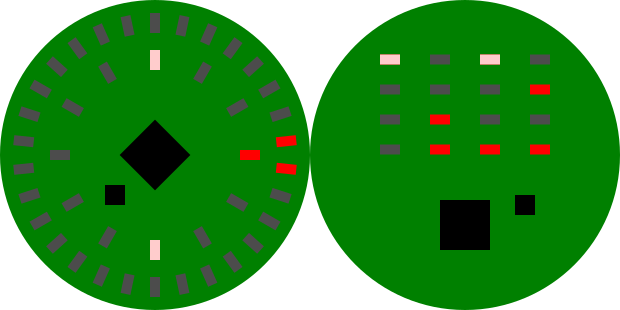
\includegraphics[width=0.6\textwidth]{../Graphics/Time3_15_debouncing}
\end{center}
Im Entprellmodus muss die Anzeige der Uhr wieder nach Oben gedreht werden und doppelt angetippt werden.
\begin{center}
\includegraphics[width=0.6\textwidth]{../Graphics/Time3_15_SetHour}
\end{center}
Im Stundeneinstellungsmodus kann die Stundenanzahl durch kippen der Uhr nach Oben (weg vom Benutzer) erhöht und durch kippen nach unten verringert werden. In der analogen Variante blinkt die LED, die normalerweise 10 Minuten anzeigt, wenn die eingestellte Stundenanzahl nach 12 Uhr mittags liegt.
Sobald die Stundenanzahl korrekt eingestellt ist kann durch doppeltippen der Minuteneinstellungsmodus aktiviert werden.
\begin{center}
\includegraphics[width=0.6\textwidth]{../Graphics/Time3_15_SetMinute}
\end{center}
der Minuteneinstellungsmodus funktioniert genau wie der Stundeneinstellungsmodus, erhöhen und verringern der Minutenanzahl kann duch kippen der Uhr erreicht werden. Wenn die Minutenanzahl richtig eingestellt ist kann der Einstellungsmodus mit doppeltippen verlassen werden. Beim Verlassen des Einstellungsmodus werden die Sekunden auf null gestellt und die Uhr beginn wieder zu laufen.
%\subsection{Read the Date}
%\begin{center}
%\includegraphics[width=0.6\textwidth]{../Graphics/Date25_Dez}
%\end{center}
%To enter the Date display mode tilt the Watch in Time Mode to the Front(Facing away from you) at least 10 degrees and double Tap it.
%\paragraph{Analog}
%On the analog Version The Minutes 40 and 50 are lit up to signal Date Display.
%On the Hours Ring the Month is displayed as Hour and the Day is Displayed as Minutes.
%
%\paragraph{Binary}
%On the binary Version the first column is showing 3 to signal Date Display.
%In the second and third column the Day is displayed as BCD Code and the Month is displayed in binary code(it does not stop on 9)\\
%\\
%A double Tap with the watch facing up switches back to show time mode.
%
%\subsubsection{setting the Date}
%To enter the Date setting mode you have to turn the Watch in show date mode upside down, Watchface facing the ground an double Tap it. The Watch enters debouncing mode.
%In debouncing mode the Hours 8 and Minutes 80 are blinking for the binary version for the Analog Version Minutes 40 and 50 are blinking. (Blinking leds are displayed brighter in the graphic.
%\begin{center}
%\includegraphics[width=0.6\textwidth]{../Graphics/Date25_Dez_debouncing}
%\end{center}
%While in debouncing mode turn the watch around again (Watchface facing up)  and double Tap it again to enter set day mode.
%\begin{center}
%\includegraphics[width=0.6\textwidth]{../Graphics/Date25_Dez_SetDay}
%\end{center}
%Setting the Day works exactly like setting the hour. Increasing and decreasing is done via leaning the Watch fowrward an backward. Once finished a double Tap switches to set month mode.
%\begin{center}
%\includegraphics[width=0.6\textwidth]{../Graphics/Date25_Dez_SetMonth}
%\end{center}
%Setting the Month works exactly like setting the hour. Increasing and decreasing is done via leaning the Watch fowrward an backward. Once finished a double Tap switches to set year mode.
%\begin{center}
%\includegraphics[width=0.6\textwidth]{../Graphics/Date25_Dez_SetYear21}
%\end{center}
%The year is only used for the leap year calculation and can be only set between 0 and 99. 
%\paragraph{Analog} 
%In the Analog Version the Set year mode is signalized by blinking both minute LEDs 30 and 50. The Year tens are shown in the inner ring with one LED per Counter and the ones are shown in the outer ring with one LED per counter. In this example XX21.
%\paragraph{Binary}
%Setting Year mode is displayed by showing 3 in the first column and blinking all LEDs in the second column. The year is displayed in columns 3 and 4. In this example XX21.\\
%\\
%Setting the Month works exactly like setting the hour. Increasing and decreasing is done via leaning the Watch fowrward an backward. Once finished a double Tap sets the Seconds to 0 and starts the Watch again.
\subsection{Anzeige der heutigen Schritte}
\begin{center}
\includegraphics[width=0.6\textwidth]{../Graphics/ShowSteps32768}
\end{center}
Um die Schrittanzeige einzuschalten muss die Uhr um etwas 10 Grad nach vorn gekippt werden und im Zeitanzeigemodus doppelt angetippt werden.

\paragraph{Analog}
In der analogen Variante wird die LED für elf Uhr gleichzeitig mit der Überlaufanzeige 0 bis 3 Uhr aktiviert. Die Überlaufanzeige zeigt die Anzahl der vollständigen Umrundung an. Eine vollständige Umrundung besteht aus 15000 Schritten.
Der äußere Ring zeigt die Schritte ohne Überlauf an. Jede LED signalisiert 500 Schritte. Der Wert wird auf 500 Schritte gerundet. Die erste Umschaltung auf die LED die normalerweise für 2 Minuten steht erfolgt also bei 251 Schritten.
In dem Beispiel ist der Überlaufzähler auf 2 und im äußeren Ring brennt die sechste LED (normalerweise 12 Minuten).
$2*15000+6*500 = 33000$
Die Anzeige signalisiert in dem Beispiel also 33000 Schritte am heutigen Tag.
\paragraph{Binary}
In der Binär Variante zeigt die erste Spalte eine 7 an, die rechten drei Spalten Zeigen die Schritte mit einer Auflösung von 100 an.
Die 32768 Schritte in dem Bispiel werden also als (7)328 angezeigt.\\
\\
Doppeltippen während die aktuellen Schritte angezeigt werden führt zurück in den Zeitanzeige Modus, wenn die Uhr nach Oben zeigt.
\subsection{Schritthistorie ansehen}
Um in den Schritthistoriemodus zu kommen muss die Uhr, während die heutigen Schritte angeszeigt werden, nach unten gedreht werden. Anschließend kann mit Doppeltippen die Schritthistorie aktiviert werden.
\begin{center}
\includegraphics[width=0.6\textwidth]{../Graphics/ShowStepsHist_2Days_ago_7500}
\end{center}
Der Historienzähler kann erhöht und verringert werden, indem die Uhr nach vorne oder nach hinten geneigt wird.
\paragraph{Analog} 
Der Schritthistorienmodus ähnelt stark der Schrittzähleranzeige. Der Einzige Unterschied ist die Anzeige des Historienzählers.
Der Historienzähler beginnt bei 4 Uhr und erhöht sich je nachdem, wie lange die zugehörige Schrittanzahl zurückliegt. In dem Beispiel ist die LED für 5 Uhr aktiviert. Damit ist die Anzeige von vor 2 Tagen. Die Schritte werden wie im Schrittzählermodus angezeigt. Die Anzeige im Beispiel zeigt also an, dass der Schrittzähler vor 2 Tagen bei 7500 lag.
\paragraph{Binary}
Die Schritthistorie wird durch die LED H80 signalisiert.
Die LEDs direkt darunter zeigen die History Counter an. Der Counter startet gestern mit 0.
Die Anzeige im Beispiel zeigt also an, dass der Schrittzähler vor 2 Tagen bei 7500 lag.\\
\\
Diese Anzeige kann mit einem Doppeltippen zur Batteriespannungsanzeige verlassen werden.
\subsection{Batteriespannungsanzeige}
Um die Battersiepannungsanzeige zu aktivieren muss im Schritthistoreinmodus ein Doppeltipp erfolgen.
\begin{center}
\includegraphics[width=0.6\textwidth]{../Graphics/ShowUBatt_2950mV}
\end{center}
\paragraph{Analog}
Die Batteriespannungsanzeige wird signalisiert, indem die Stundenanzeige für 11 und 12 Uhr gemeinsam angezeigt wird.
Die Batterispannung wird auf dem äußeren Ring skaliert von 3,5V bis 1,5V angezeigt. Jedes Viertel entspricht also 0,5V.
Die Uhr in dem Beispiel zeigt also 2,95V an.

\paragraph{Binary}
Die Batteriespannungsanzeige wird durch die LED H40 signalisiert.
Die rechten 3 Spalten zeigen die Batteriespannung in 10mV Schritten an.
$2950mV=2,95V$\\
\\
Doppeltippen in diesem Modus führt zurück in den Schrittanzeigemodus.